% Бүлэг 2

\chapter{СИСТЕМИЙН ШААРДЛАГА ТОДОРХОЙЛОХ, ШИНЖИЛГЭЭ ХИЙХ} % Зарим нэг зөвлөмж

\label{Chapter2} % Энэ бүлэг рүү ишлэл хийх бол \ref{Chapter2} командыг ашигла 
\pagecolor{white}
%-------------------------------------------------------------------------------
%	SECTION 1
%-------------------------------------------------------------------------------
\textbf{Системийн үйл ажиллагааны тухай дэлгэрэнгүй}\\
Энэхүү вэб систем нь бүжгийн спортоор хичээллэхийг хүссэн хүн бүхэнд зориулсан, бүжгийн төрөл болон анхан, дунд, гүнзгий шатны сургалтуудыг агуулсан бөгөөд суралцах хүсэлтэй хэн бүхэнд зориулсан байх болно. \\
Бүжгийн спорт, цахим сургалтын вэб систем нь бүртгүүлсэн хэрэглэгч өөрийн бүртгэлийн ангилалаас хамааран бүжгийн сургалтыг онлайнаар, танхимаар болон хосолсон байдлаар сургалтанд хамрагдах боломжтой болно. Онлайн сургалтыг сонгосон хэрэглэгч өөрийн хүссэн үедээ цахим төхөөрөмжөө ашиглан урьдчилан бэлдсэн сургалтандаа хамрагдах боломжтой. Танхимын сургалтанд бүртгүүлсэн хэрэглэгч сургалтын төрөл болон цагаа сонгож сургалтандаа хамрагдана. Хосолсон хэлбэрийн хэрэглэгчид нь дээрх 2 эрхийг давхар эзэмших эрхтэй байна. Админ хэрэглэгч нь шинэ хэрэглэгчийн бүртгэлийг шалгаж, төлбөр болон танхимын сургалтын өдөр цагийг баталгаажуулна. Мөн дараа дараагийн шинэ видео хичээлүүдийг вэб сайтад байрлуулна.
\section{Системийг ашиглах хэрэглэгчид}
Энэхүү вэб нь Админ болон хэрэглэгч гэсэн 2 оролцогчтой. Хэрэглэгч нь дотроо гурван ангилалд хуваагдана. 
\begin{itemize}
    \item [•] Админ нь: Системд хэрэглэгч бүртгэх, хасах, хэрэглэгчийн эрхийг баталгаажуулах, шинэ онлайн хичээлүүдийг нэмэх үүрэгтэй
    \item [•] Онлайн хэрэглэгч: Вэбд байрласан хичээлээс өөрийн сонгосон төрлийн хичээлийг цахим төхөөрөмжөө ашиглан хүссэн үедээ үзэж судлах эрхтэй
    \item [•] Танхим хэрэглэгч: Сонгосон цагийн хуваарийн дагуу сургалтандаа хамрагдах эрхтэй
    \item [•] Хосолсон хэрэглэгч: Танхимд сонгосон цагийн хуваарийн дагуу хичээлдээ хамрагдан суралцахаас гадна онлайнаар видео хичээлийг үзэх давхар эрхтэй байна. 
\end{itemize}
\section{Функционал шаардлага}
\begin{itemize}
    \item [1.] Админы функционал шаардлага:
\end{itemize}
\begin{itemize}
    \item [1.1.] Системд нэвтрэх
    \item [1.2.] Хэрэглэгч бүртгэх
    \item [1.3.] Хэрэглэгчдийг ангилж, баталгаажуулах
    \item [1.4.] Хэрэглэгчдийн төлөвийг хянах
    \item [1.5.] Онлайн сургалтыг удирдах
    \item [1.6.] Онлайн сургалтыг нэмэх
\end{itemize}
\begin{itemize}
    \item [2.] Онлайн хэрэглэгчийн функционал шаардлага:
\end{itemize}
\begin{itemize}
    \item [2.1.] Системд нэвтрэх
    \item [2.2.] Бүжгийн төрлөө сонгож бүртгүүлэх
    \item [2.3.] Сонгосон бүжгийн төрлийн видео хичээлүүдийг харах
    \item [2.4.] Давхар сургалтанд бүртгүүлэх
    \item [2.5.] Хэрэглэгчийн ангилалаа солих
\end{itemize}
\begin{itemize}
    \item [3.] Танхимын хэрэглэгчийн функционал шаардлага:
\end{itemize}
\begin{itemize}
    \item [3.1.] Системд нэвтрэх
    \item [3.2.] Бүжгийн төрлөө сонгож бүртгүүлэх
    \item [3.3.] Сонгосон цагийн хуваарийн дагуу танхимд хичээллэх
    \item [3.4.] Хэрэглэгчийн ангилалаа солих
\end{itemize}
\begin{itemize}
    \item [4.] Хосолсон хэрэглэгчийн функционал шаардлага:
\end{itemize}
\begin{itemize}
    \item [4.1.] Системд нэвтрэх
    \item [4.2.] Бүжгийн төрлөө сонгож бүртгүүлэх
    \item [4.3.] Сонгосон бүжгийн төрлийн видео хичээлүүдийг харах
    \item [4.4.] Сонгосон цагийн хуваарийн дагуу танхимд хичээллэх
    \item [4.5.] Давхар сургалтанд бүртгүүлэх
    \item [4.6.] Хэрэглэгчийн ангилалаа солих
\end{itemize}
\section{Функционал бус шаардлага}
\begin{itemize}
    \item [1.] Гүйцэтгэлийн шаардлага:
\end{itemize}
\begin{itemize}
    \item [1.1.] Өгөгдлийн сан ачааллах хугацаа нь хурдан шуурхай байх
    \item [1.2.] Өгөгдлийн сангийн зохион байгуулалт оновчтой байх
    \item [1.3.] Хэрэглэгчийн интерфейс энгийн ойлгомжтой байх
\end{itemize}
\begin{itemize}
    \item [2.] Аюулгүй байдлын шаардлага:
\end{itemize}
\begin{itemize}
    \item [2.1.] Серверийн аюулгүй байдлыг хангасан байх
    \item [2.2.] Хэрэглэгчийн нэвтрэх хэсэг аюулгүй байх
    \item [2.3.] Хэрэглэгчийн хувийн мэдээлэл аюулгүй байх
    \item [2.4.] Системийн аюулгүй байдлыг хангасан ӨСУС ашигладаг байх
    \item [2.5.] Системийн хэрэглэгчдийг санаатай эсвэл санамсаргүй байдлаар систем гэмтээх, өөрт харьяалалгүй мэдээллийг устгах, хандах, өөрчлөхөөс сэргийлсэн байх.
\end{itemize}
\begin{itemize}
    \item [3.] Хамгаалалт, нууцлалын шаардлага:
\end{itemize}
\begin{itemize}
    \item [3.1.] Хэрэглэгчийн мэдээллийг нууцлалтай хадгалах
    \item [3.2.] Дэлгэцэнд нууц үг харуулдаггүй байх
\end{itemize}
\begin{itemize}
    \item [4.] Техникийн шаардлага:
\end{itemize}
\begin{itemize}
    \item [4.1.] Вэб систем нь бүх төрлийн вэб хөтөч ашиглах боломжтой байх
\end{itemize}
\section{Юзкейс диаграм}
\begin{figure}[ht]
    \centering
    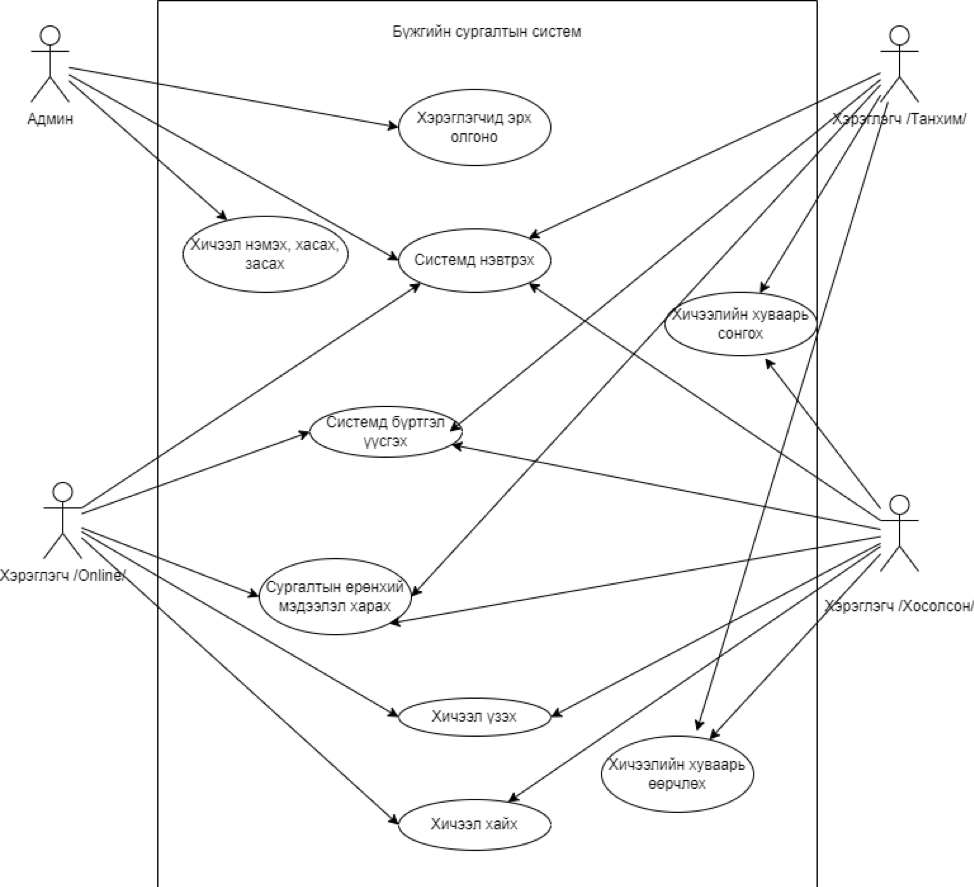
\includegraphics[scale=0.9]{Figures/pic21.png}
    \caption{Админ болон хэрэглэгчийн юзкейс диаграм}
    \label{fig21}
\end{figure}
\newpage
\section{Юзкейс диаграмын тодорхойлолт}
\begin{table}[hp!]
    \centering
    \begin{tabular}{|c|p{10cm}|}
    \hline
    Нэр: & Системд нэвтрэх \\ \hline
    ID: & 1 \\ \hline
    Үүсгэсэн:	& Д.Бат \\ \hline
    Үүсгэсэн огноо:&	2023.05.24 \\ \hline
    Товч тайлбар: &  Програмын хэрэглэгчид системд нэвтэрнэ\\ \hline
    Үндсэн оролцогч: & 1. Админ, 2. Хэрэглэгч\\ \hline
    Хоёрдох оролцогч:	&Байхгүй \\ \hline
    Өмнөх нөхцөл:	&	Систем хэвийн ажиллагаатай байх \\ \hline
    Үндсэн урсгал:	& 1.	Админ, хэрэглэгч системд нэвтрэхийг хүссэнээр энэ юзкейс эхэлнэ \\ 
    &2.	Систем нэвтрэх форум харуулна\\
    &3.	Хэрэглэгч нэвтрэх нэр, нууц үг оруулна\\
    &4.	Системд нэвтрэх эрхийг шалгана\\
    &5.	Хэрэв нэвтрэх нууц үг буруу бол алдаа илгээнэ\\
    & 6.	Нэвтрэх нэр, нууц үг зөв бол систем нэвтрэх үйлдлийг гүйцэтгэнэ \\ \hline
    Дараах нөхцөл:	&	Програмын хэрэглэгчид системд нэвтэрсэн байна \\ \hline
    Альтернатив урсгал:&	1.	Нэвтрэх нэр, нууц үг буруу байна\\
    & 2.	Веб системд алдаа гарсан \\ \hline
    \end{tabular}
    \caption{Системд нэвтрэх}
    \label{tab21}
\end{table}
\begin{table}[bp!]
    \centering
    \begin{tabular}{|c|p{10cm}|}
    \hline
    Нэр:	&Хэрэглэгчид эрх олгох \\ \hline
    ID:&	2 \\ \hline
    Үүсгэсэн:&	Д.Бат \\ \hline
    Үүсгэсэн огноо:	&2023.05.24 \\ \hline
    Товч тайлбар:	&Админ хэрэглэгчийн мэдээллийг бүртгэнэ \\ \hline
    Үндсэн оролцогч:	&1.	Админ \\ \hline
    Хоёрдох оролцогч:	&Байхгүй \\ \hline
    Өмнөх нөхцөл:&	1.	Систем хэвийн ажиллагаатай байх\\
    &2.	Админ өөрийн эрхээр нэвтэрч орсон байх\\
    &3.	Хэрэглэгч нөхцөлийг хангасан байх\\ \hline
    Үндсэн урсгал:	&1.	Админ хэрэглэгчийн мэдээллийн хэсгийг сонгосноор энэ юзкейс эхэлнэ \\ \hline
    &2.	Хэрэв админ хэрэглэгчид сургалтын эрх олгох бол \\ \hline
    &3.	Систем хэрэглэгчдийн мэдээллийг харуулна \\ \hline
    &4.	Админ тухайн хэрэглэгчийн сургалтын төрлийг сонгож хадгална \\ \hline
    Дараах нөхцөл:	& 1.	Хэрэглэгчид эрх олгогдсон байна \\
    & 2. 	Хэрэглэгчийн эрх хасагдсан байна \\ \hline
    Альтернатив урсгал:	& 1. Веб системийн алдаа гарсан \\ \hline
    \end{tabular}
    \caption{Хэрэглэгчид эрх олгох}
    \label{tab22}
\end{table}

\begin{table}[hp!]
    \centering
    \begin{tabular}{|c|p{10cm}|}
    \hline
    Нэр:&	Хичээл хайх \\ \hline
    ID:	&3 \\ \hline
    Үүсгэсэн:	&Д.Бат \\ \hline
    Үүсгэсэн огноо:&	2023.05.24 \\ \hline
    Товч тайлбар:	&Админ, хэрэглэгч хичээл хайх \\ \hline
    Үндсэн оролцогч:&	1.	Админ  \\
    &2.	Хэрэглэгч \\ \hline
    Хоёрдох оролцогч:	&Байхгүй \\ \hline
    Өмнөх нөхцөл:&	1.	Систем хэвийн үйл ажиллагаатай байх \\ \hline
    Үндсэн урсгал:&	1.	Админ, хэрэглэгч хичээл хайх хэсгийг сонгосноор энэ юзкейс эхэлнэ.\\
    &2.	Хэрэглэгч хичээл хайх бол\\
    &3.	Систем хичээл хайх талбарыг харуулна\\
    &4.	Хэрэглэгчид хичээл хайна\\
    &5.	Хэрэв хичээл хайх талбар хоосон бол\\
    &5.1 Систем алдааны мессеж илгээнэ\\
    &6.	Систем хайлтын үр дүнг харуулна\\ \hline
    Дараах нөхцөл:	& 1.	Хэрэглэгч хичээл хайсан \\ \hline
    Альтернатив урсгал:	&1.	Веб систем алдаа гарсан\\
    &2.	Хайсан хичээлийн утга буруу\\ \hline
    \end{tabular}
    \caption{Хичээл хайх}
    \label{tab23}
\end{table}
\begin{table}[bp!]
    \centering
    \begin{tabular}{|c|p{10cm}|}
    \hline
    Нэр:&	Хичээл нэмэх \\ \hline
    ID:&	4 \\ \hline
    Үүсгэсэн:&	Д.Бат \\ \hline
    Үүсгэсэн огноо:	&2023.05.24 \\ \hline
    Товч тайлбар:	&Админ системд хичээл нэмнэ \\ \hline
    Үндсэн оролцогч:&	1.	Админ \\ \hline
    Хоёрдох оролцогч:	&Байхгүй \\ \hline
    Өмнөх нөхцөл:	&1.	Систем хэвийн үйл ажиллагаатай байх\\
    &2.	Админ системд нэвтэрсэн байх\\ \hline
    Үндсэн урсгал:&	1.	Админ хичээл нэмэх хэсгийг сонгосноор энэ юзкейс эхэлнэ\\
    &2.	Админ хичээл байршуулах бол\\
    &3.	Систем хичээлийн мэдээллийг оруулах талбарыг харуулна\\
    &4.	Админ хичээлийн мэдээллийг харуулна\\
    &5.	Систем хичээлийн мэдээллийг бүртгэн авна\\
    &6.	Систем хичээлийг нэмж оруулсан мессеж илгээнэ\\ \hline
    Дараах нөхцөл:	&1.	Админ системд хичээл байршуулсан \\ \hline
    Альтернатив урсгал:	&Веб систем алдаа гарсан \\ \hline
    \end{tabular}
    \caption{Хичээл нэмэх}
    \label{tab24}
\end{table}

\begin{table}[hp!]
    \centering
    \begin{tabular}{|c|p{10cm}|}
    \hline
    Нэр:&	Хичээл засах, хасах\\ \hline
    ID:&	5\\ \hline
    Үүсгэсэн:&	Д.Бат\\ \hline
    Үүсгэсэн огноо:	&2023.05.24\\ \hline
    Товч тайлбар:&	Админ байршуулсан хичээлийг засна, устгана.\\ \hline
    Үндсэн оролцогч:&	1.	Админ\\ \hline
    Хоёрдох оролцогч:	&Байхгүй\\ \hline
    Өмнөх нөхцөл:	&1.	Систем хэвийн үйл ажиллагаатай байх\\
         &   2.	Админ системд нэвтэрсэн байх\\ \hline
    Үндсэн урсгал:	&1.	Админ хичээл удирдах хэсгийг сонгосноор энэ юзкейс эхэлнэ\\
    &2.	Админ хичээлийн мэдээллийг засах бол\\
    &3.	Систем хичээлийн мэдээллийг засах талбарыг харуулна\\
    &4.	Админ хичээлийн мэдээллийг засна\\
    &5.	Систем хичээлийн мэдээлэл засагдсан мессеж илгээнэ\\
    &6.	Админ хичээлийн мэдээллийг устгах бол\\
    &7.	Систем хичээлийн мэдээллийг устгах талбарыг харуулна\\
    &8.	Админ хичээлийн мэдээллийг устгана\\
    &9.	Систем хичээлийн мэдээллийг устгагдсан мессеж илгээнэ\\ \hline
    Дараах нөхцөл:	&1.	Хичээл засагдсан\\
    &2.	Хичээл устгагдсан\\ \hline
    Альтернатив урсгал:	& Веб систем алдаа гарсан\\ \hline
    \end{tabular}
    \caption{Хичээл засах, хасах}
    \label{tab25}
\end{table}
\begin{table}[bp!]
    \centering
    \begin{tabular}{|c|p{10cm}|}
    \hline
    Нэр:&	Системд бүртгэл үүсгэх\\ \hline
    ID:&	6\\ \hline
    Үүсгэсэн:&	Д.Бат\\ \hline
    Үүсгэсэн огноо:	&2023.05.24\\ \hline
    Товч тайлбар:&	Хэрэглэгч системд бүртгэл үүсгэнэ\\ \hline
    Үндсэн оролцогч:&	1.	Хэрэглэгч\\ \hline
    Хоёрдох оролцогч:&	Байхгүй\\ \hline
    Өмнөх нөхцөл:&	1.	Систем хэвийн үйл ажиллагаатай байх\\ \hline
    Үндсэн урсгал:&	1.	Хэрэглэгч бүртгэл үүсгэх хэсэг рүү орсноор энэ юзкейс эхэлнэ\\
   & 2.	Систем бүртгүүлэх форм харуулна\\
   & 3.	Хэрэглэгч хувийн мэдээлэл болон нууц үг оруулна \\
    &4.	Систем хэрэглэгчийг бүртгэж авна\\
    &5.	Систем хэрэглэгчийг бүртгэсэн мессеж илгээнэ\\ \hline
    Дараах нөхцөл:&	1.	Хэрэглэгчийн бүртгэл үүссэн\\ \hline
    Альтернатив урсгал:	&Веб систем алдаа гарсан\\ \hline
    \end{tabular}
    \caption{Системд бүртгэл үүсгэх}
    \label{tab26}
\end{table}

\begin{table}[hp!]
    \centering
    \begin{tabular}{|c|p{10cm}|}
    \hline
    Нэр: & Сургалтын мэдээлэл харах \\ \hline
    ID: & 7 \\ \hline
    Үүсгэсэн:	 & Д.Бат \\ \hline
    Үүсгэсэн огноо:	 & 2023.05.24 \\ \hline
    Товч тайлбар: & 	Хэрэглэгч сургалтын мэдээллийг харах \\ \hline
    Үндсэн оролцогч: & 	1.	Хэрэглэгч \\ \hline
    Хоёрдох оролцогч: & 	Байхгүй \\ \hline
    Өмнөх нөхцөл:	 & 1.	Систем хэвийн үйл ажиллагаатай байх\\
     & 2.	Хэрэглэгч системд нэвтэрч орсон байх \\ \hline
    Үндсэн урсгал: & 	1.	Хэрэглэгч сургалтын дэлгэрэнгүй мэдээллийг харах хэсгийг сонгосноор энэ юзкейс эхэлнэ\\
    &  2.	Хэрэглэгч сургалтын дэлгэрэнгүй мэдээллийг харах бол\\
     & 3.	Систем сургалтын дэлгэрэнгүй мэдээллийг харуулна \\ \hline
    Дараах нөхцөл:	 & 1.	Сургалтын дэлгэрэнгүй мэдээллийг харна \\ \hline
    Альтернатив урсгал:	 & Веб систем алдаа гарсан \\ \hline
    \end{tabular}
    \caption{Сургалтын мэдээлэл харах}
    \label{tab27}
\end{table}
\begin{table}[bp!]
    \centering
    \begin{tabular}{|c|p{10cm}|}
    \hline
    Нэр:	& Хичээл үзэх\\ \hline
    ID:& 	8\\ \hline
    Үүсгэсэн:	& Д.Бат\\ \hline
    Үүсгэсэн огноо:	& 2023.05.24\\ \hline
    Товч тайлбар:	& Хэрэглэгч хичээл үзэх\\ \hline
    Үндсэн оролцогч:	& 1.	Хэрэглэгч\\ \hline
    Хоёрдох оролцогч:& 	Байхгүй\\ \hline
    Өмнөх нөхцөл:	& 1.	Систем хэвийн үйл ажиллагаатай байх\\
    & 2.	Хэрэглэгч системд нэвтэрч орсон байх\\
    & 3.	Хэрэглэгч онлайн сургалтын төрлийг сонгон баталгаажуулсан байх\\ \hline
    Үндсэн урсгал:	& 1.	Хэрэглэгч хичээл үзэх хэсгийг сонгосноор энэ юзкейс эхэлнэ\\
    & 2.	Хэрэглэгч хичээл сонгож үзэх бол\\
    & 3.	Систем хичээлийн жагсаалт харуулна\\
    & 4.	Хэрэглэгч хичээлээ сонгож үзнэ\\ \hline
    Дараах нөхцөл:& 	1.	Хэрэглэгч хичээл үзнэ\\ \hline
    Альтернатив урсгал:	& Веб систем алдаа гарсан\\ \hline
    \end{tabular}
    \caption{Хичээл үзэх}
    \label{tab28}
\end{table}

\begin{table}[hp!]
    \centering
    \begin{tabular}{|c|p{10cm}|}
    \hline
    Нэр:&	Хичээлийн хуваарь сонгох \\ \hline
    ID:	&9\\ \hline
    Үүсгэсэн:&	Д.Бат\\ \hline
    Үүсгэсэн огноо:&	2023.05.24\\ \hline
    Товч тайлбар:&	Хэрэглэгч танхимаар орох хичээлийн хуваарь сонгох\\ \hline
    Үндсэн оролцогч:&	1.	Хэрэглэгч\\ \hline
    Хоёрдох оролцогч:&	Байхгүй\\ \hline
    Өмнөх нөхцөл:	&1.	Систем хэвийн үйл ажиллагаатай байх\\
   & 2.	Хэрэглэгч системд нэвтэрч орсон байх\\
    &3.	Хэрэглэгч сургалтын төрөл (танхим, хосолсон)-ийг сонгон баталгаажуулсан байх\\ \hline
    Үндсэн урсгал:&	1.	Хэрэглэгч хуваарь сонгох хэсгийг сонгосноор энэ юзкейс эхэлнэ\\
   & 2.	Хэрэглэгч хуваарь сонгох бол\\
    &3.	Систем хичээлийн хуваариудыг харуулна\\
    &4.	Хэрэглэгч хичээлийн хуваарийг сонгож хадгална\\
    &5.	Систем хуваарь амжилттай сонгогдсон мессеж илгээнэ\\ \hline
    Дараах нөхцөл:	&1.	Хэрэглэгч танхимын хичээлийн хуваарь сонгоно\\ \hline
    Альтернатив урсгал:&	1.	Веб систем алдаа гарсан\\
    &2.	Тухайн хичээлийн хуваарьт анги дүүрсэн\\ \hline
    \end{tabular}
    \caption{Хичээлийн хуваарь сонгох}
    \label{tab29}
\end{table}
\begin{table}[bp!]
    \centering
    \begin{tabular}{|c|p{10cm}|}
    \hline
    Нэр:&	Хичээлийн хуваарь өөрчлөх \\ \hline
    ID:&	10\\ \hline
    Үүсгэсэн:	&Д.Бат\\ \hline
    Үүсгэсэн огноо:	&2023.05.24\\ \hline
    Товч тайлбар:	&Хэрэглэгч хичээлийн хуваарийг өөрчлөх\\ \hline
    Үндсэн оролцогч:&	1.	Хэрэглэгч\\ \hline
    Хоёрдох оролцогч:	&Байхгүй\\ \hline
    Өмнөх нөхцөл:	&1.	Систем хэвийн үйл ажиллагаатай байх\\
    &2.	Хэрэглэгч системд нэвтэрч орсон байх\\
    &3.	Хэрэглэгч сургалтын төрөл (танхим, хосолсон)-ийг сонгон баталгаажуулсан байх\\
    &4.	Хэрэглэгч өмнө нь хичээл сонгосон байх\\ \hline
    Үндсэн урсгал:	&1.	Хэрэглэгч хуваарь сонгох хэсгийг сонгосноор энэ юзкейс эхэлнэ\\
    &2.	Хэрэглэгч хуваарь өөрчлөх бол\\
    &3.	Систем өөрчлөх боломжтой хичээлийн хуваариудыг харуулна\\
    &4.	Хэрэглэгч хичээлийн хуваарийг сонгож хадгална\\
    &5.	Систем хуваарь амжилттай өөрчлөгдсөн мессеж илгээнэ\\ \hline
    Дараах нөхцөл:	&1.	Хэрэглэгч танхимын хичээлийн хуваарь өөрчилнө\\ \hline
    Альтернатив урсгал:	&Веб систем алдаа гарсан\\ \hline
    \end{tabular}
    \caption{Хичээлийн хуваарь өөрчлөх}
    \label{tab210}
\end{table}

